\section{Solution procedures for nonlinear systems}
We illustrate this on problem of nonlinear mechanics. Our starting point is general form of equilibrium equations expressing the balance between internal $\mbf{f}^{int}$ and external $\mbf{f}^{ext}$
$$
\mbf{f}^{int}(\mbf{r}) = \mbf{f}^{ext}
$$
Suppose we are looking for an equilibrium at the end of load increment $\Delta\mbf{f}^{ext}$
\begin{equation}
  \mbf{f}^{int}(\mbf{r}+\Delta\mbf{r}) = \mbf{f}^{ext}+\Delta\mbf{f}^{ext}
  \label{eq:nonlinearequalibrium}
\end{equation}
By the linearization of the nodal force vector around known equilibrium state we can obtain
\begin{equation}
  \mbf{f}^{int}(\mbf{r})+\pard{\mbf{f}^{int}}{\mbf{r}}\Delta\mbf{r}+O(\|\Delta\mbf{r}\|^2)
\end{equation}
The derivative of internal force vector with respect to nodal displacements is called jacobian matrix and in solid mechanics as tangent stiffness matrix.
For the case of material non-linearity
$$
\mbf{f}^{e,int}(\mbf{r^e})=\int_{\Omega^e}\mbf{B}^T\mbf{\sigma}(\mbf{\eps}(\mbf{r^e}))\ d\Omega \Rightarrow
\pard{\mbf{f}^{e,int}}{\mbf{d}^e} = \int_{\Omega^e}\mbf{B}^T\pard{\mbf{\sigma}}{\mbf{\eps}}\pard{\mbf{\eps}}{\mbf{r^e}}\ d\Omega =
\int_{\Omega^e}\mbf{B}^T\pard{\mbf{\sigma}}{\mbf{\eps}}\mbf{B}{\mbf{r}^e}\ d\Omega =
\int_{\Omega^e}\mbf{B}^T\mbf{D}\mbf{B}{\mbf{r}^e}\ d\Omega
\label{eq:newtonlinearization}
$$

\subsection{Newton-Raphson method}
The method is based on splitting of the loading process into series of subsequent incremental loading steps in which the incremental loading vector $\Delta\mbf{f}$ is applied. We are looking for the equilibrium at the end of loading step~\ref{eq:nonlinearequalibrium} using the iterative procedure outlined in~\ref{eq:newtonlinearization}. The algorithm is graphically outlined in Fig.~\ref{fig:newtonraphson} for a system with one unknown and summarized in Table~\ref{tab:newtonraphson}.

\begin{figure}
  \begin{center}
    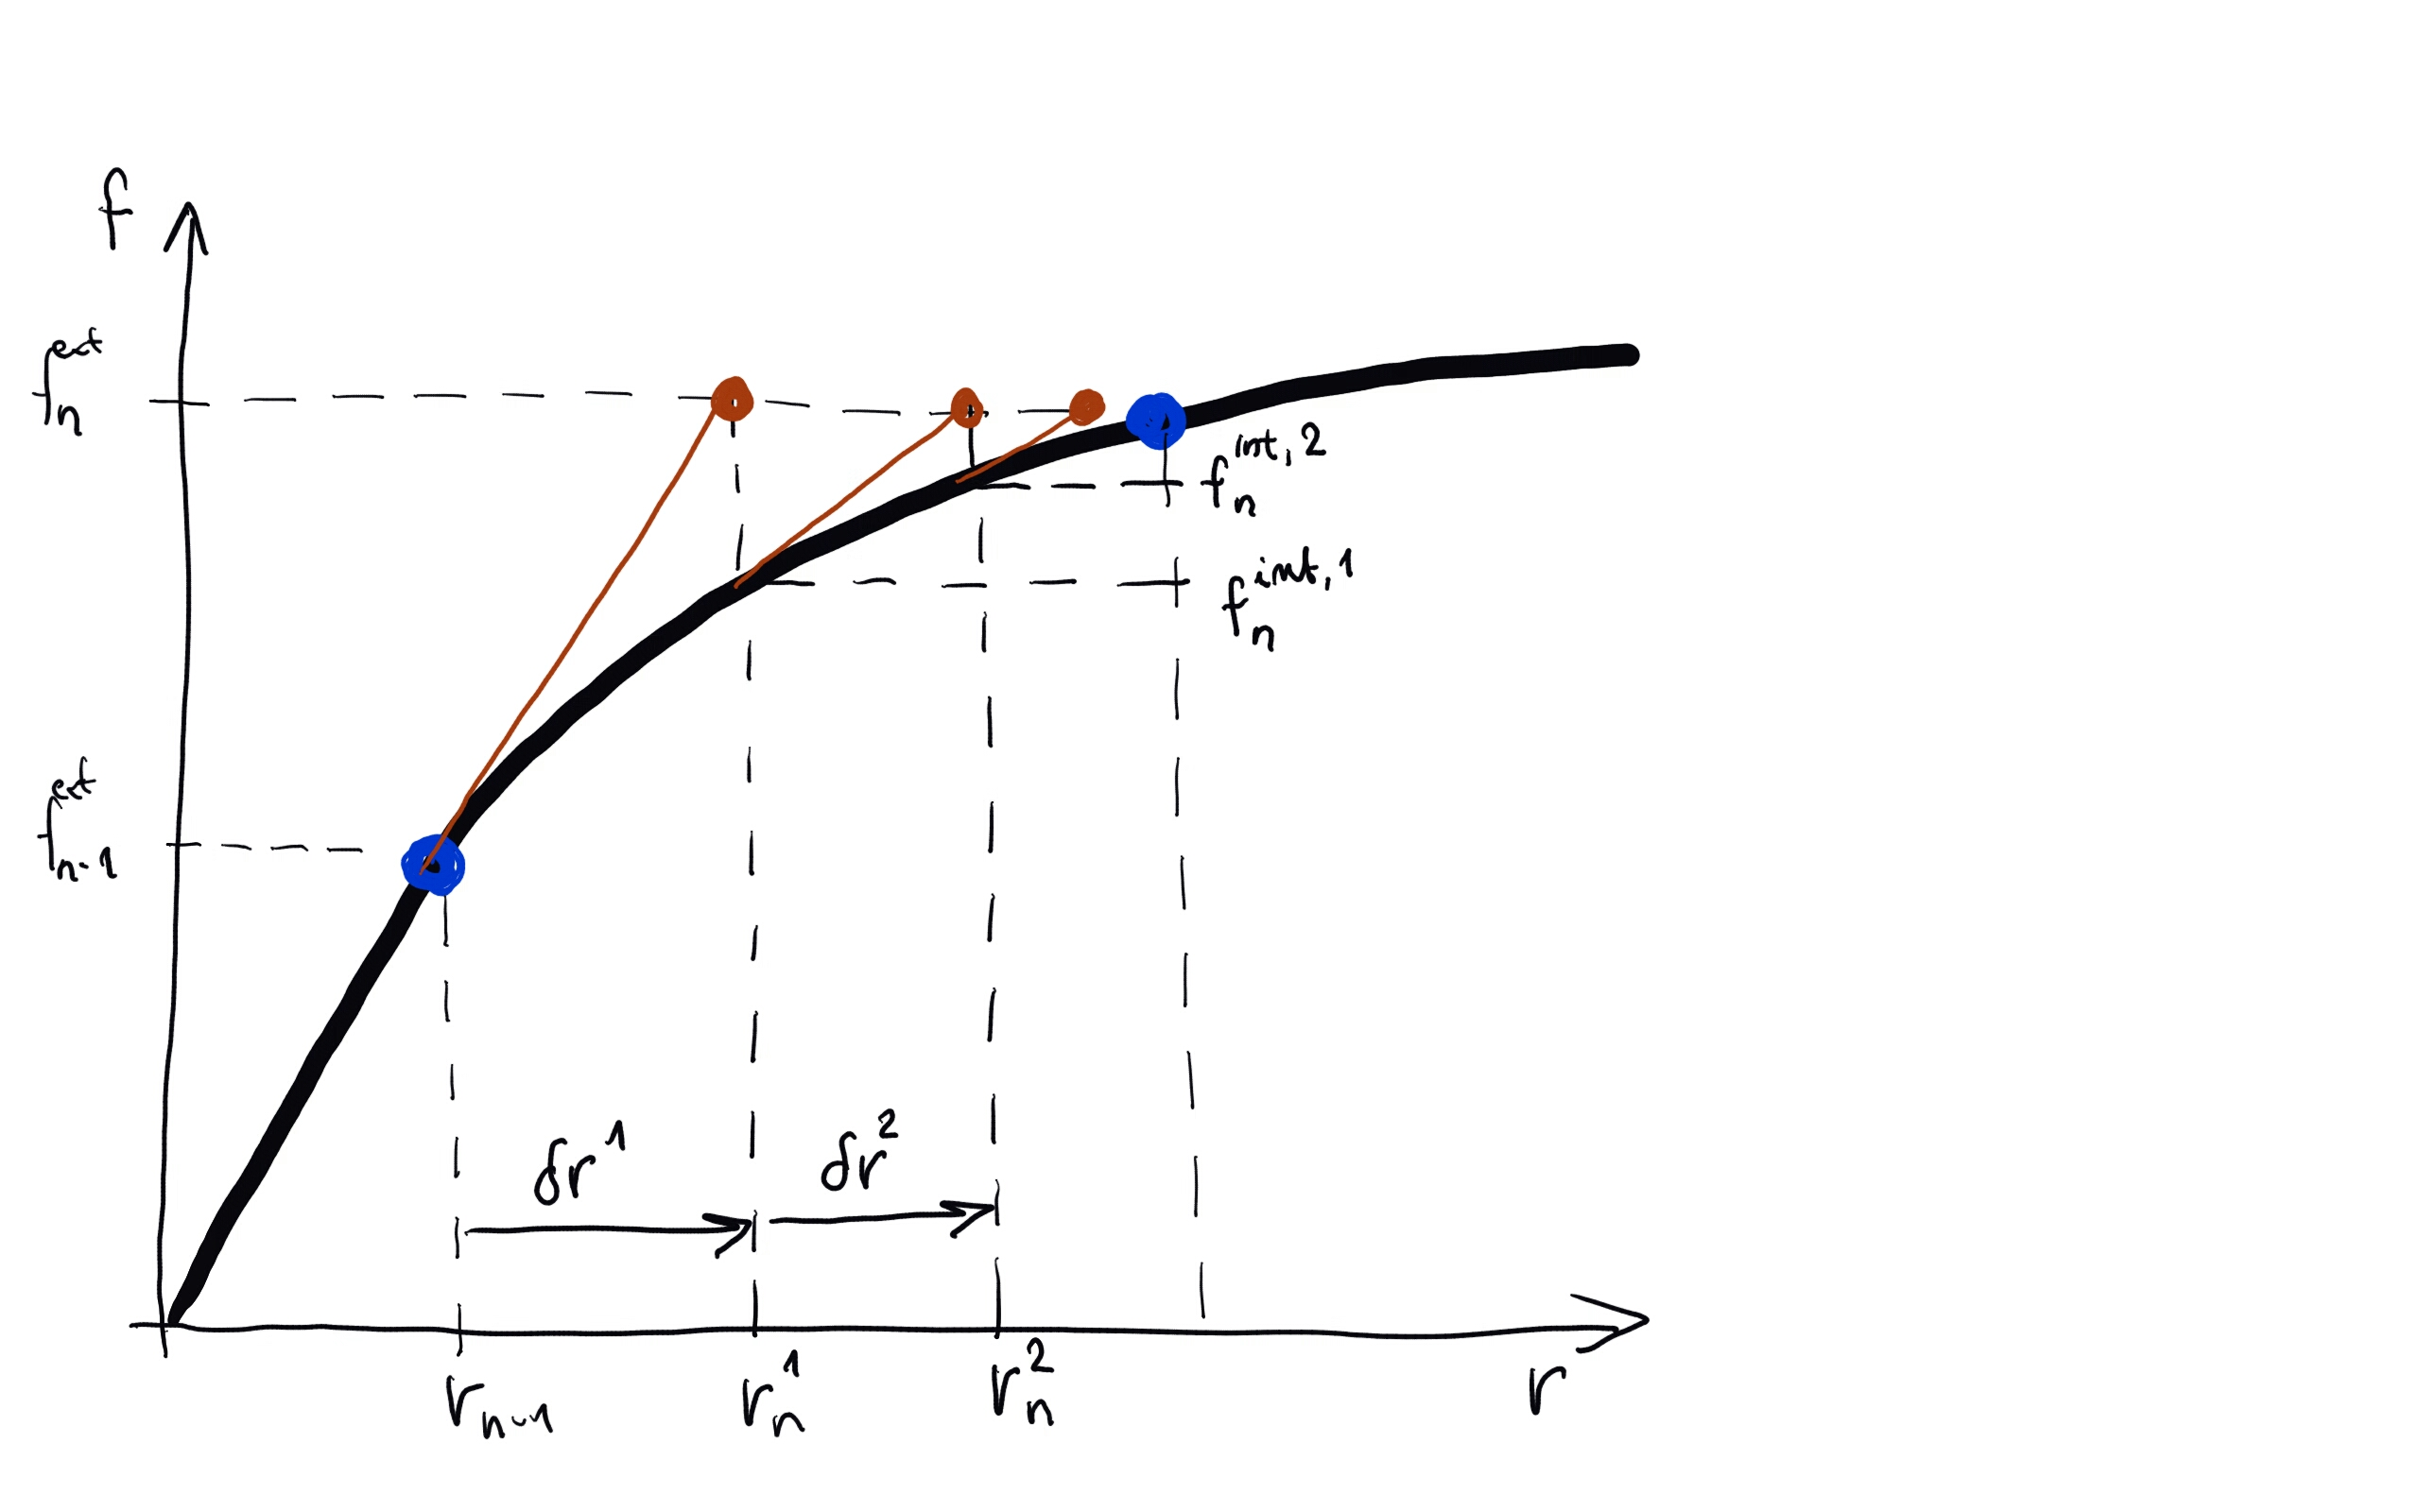
\includegraphics[width=0.8\textwidth]{figs/newtonraphson.png}
  \end{center}
  \label{fig:newtonraphson}
  \caption{Illustration of Newton-Raphson method}
\end{figure}


\begin{table}[h!]
  \begin{center}
  \begin{tabular}{|l|l|}
    \hline
    Given \\
    \;\;$\mbf{f}^{ext}_{n-1}$\\
    \;\;$\mbf{f}^{ext}_{n}=\mbf{f}^{ext}_{n-1}+\delta\mbf{f}^{ext}_n$\\
    \;\;$\mbf{r}^{0}_{n} = \mbf{r}_{n-1}$\\
    Looking for $\mbf{r}_n$, such that $\mbf{f}^{int}(\mbf{r}_n) = \mbf{f}^{ext}_n$\\
    Solve for $i=1,2,\cdots$\\ 
    \;\;$\mbf{K}^{i}\delta\mbf{r}^{i} = \mbf{f}^{ext}_n-\mbf{f}^{int}_n(\mbf{r}^{i-1}_{n})$\\
    \;\;$\mbf{r}^i_{n} = \mbf{r}^{i-1}_{n}+\delta\mbf{r}^i$\\
    Until $\|\mbf{f}^{ext}_n-\mbf{f}^{int}_n(\mbf{r}^{i-1}_{n})\| \le \eps$\\
    \hline
  \end{tabular}
  \end{center}
  \caption{Newton-Raphson method}
  \label{tab:newtonraphson}
\end{table}

Based on update strategy for stiffness matrix, one can obtain different variants of the method. 
When the stiffness matrix $\mbf{K}^{i}$ is updated in each iteration, the full Newton-Raphson method is obtained. When stiffness matrix only every n-th iteration, one speaks about modified Newton-Raphson method. Finally, when the stiffness matrix is updated only at the beginning of the loading step, one obtains so called initial stiffness method.
For the full Newton-Raphson method a quadratic convergence is obtained.

One can implement two blends of Newton-Raphson algorithm, where the loading can be driven by load control or by displacement control, where the prescribed increments of displacements are applied to selected DOFs.

\subsection{Arc-length method}
We start by assuming the parametrized loading, in which the total external load vector is expressed as 
$$\mbf{f}^{ext}(\lambda) = +\lambda\mbf{f}^{ext}_p$$
where $\mbf{f}_p$ is proportional, reference load vector, and $\lambda$ is load scaling parameter, 
The arc-length method is based on idea of controlling the length passed along the loading path. For the differential length of loading  path we can write
\begin{equation}
  \Delta l = \sqrt{\Delta\mbf{r}^T\Delta\mbf{r}+(c^2\Delta\lambda^2\mbf{f}^T_p\mbf{f}_p)}
  \label{eq:arclength}
\end{equation}
where $c$ is coefficient of generalized metrics used to define $\Delta l$ (taking into account different units of displacement and load).
For selected increment of loading path length $\Delta l$, we are looking for the equilibrium, where the unknowns are nodal displacements $\mbf{r}$ and the load scaling parameter $\lambda$. We have the equilibrium equation and additional scalar equation~\ref{eq:arclength}:
\begin{eqnarray}
  \label{eq:alm1}
  \mbf{f}^{int}(\mbf{r}_n) &=& \mbf{f}^{ext}(\lambda_n\mbf{f}_p)\\
  \label{eq:alm2}
  \Delta l_n^2&=&\Delta\mbf{r}_n^T\Delta\mbf{r}_n+c^2\Delta\lambda^2\mbf{f}^T_p\mbf{f}_p
\end{eqnarray}

\begin{figure}
  \begin{center}
    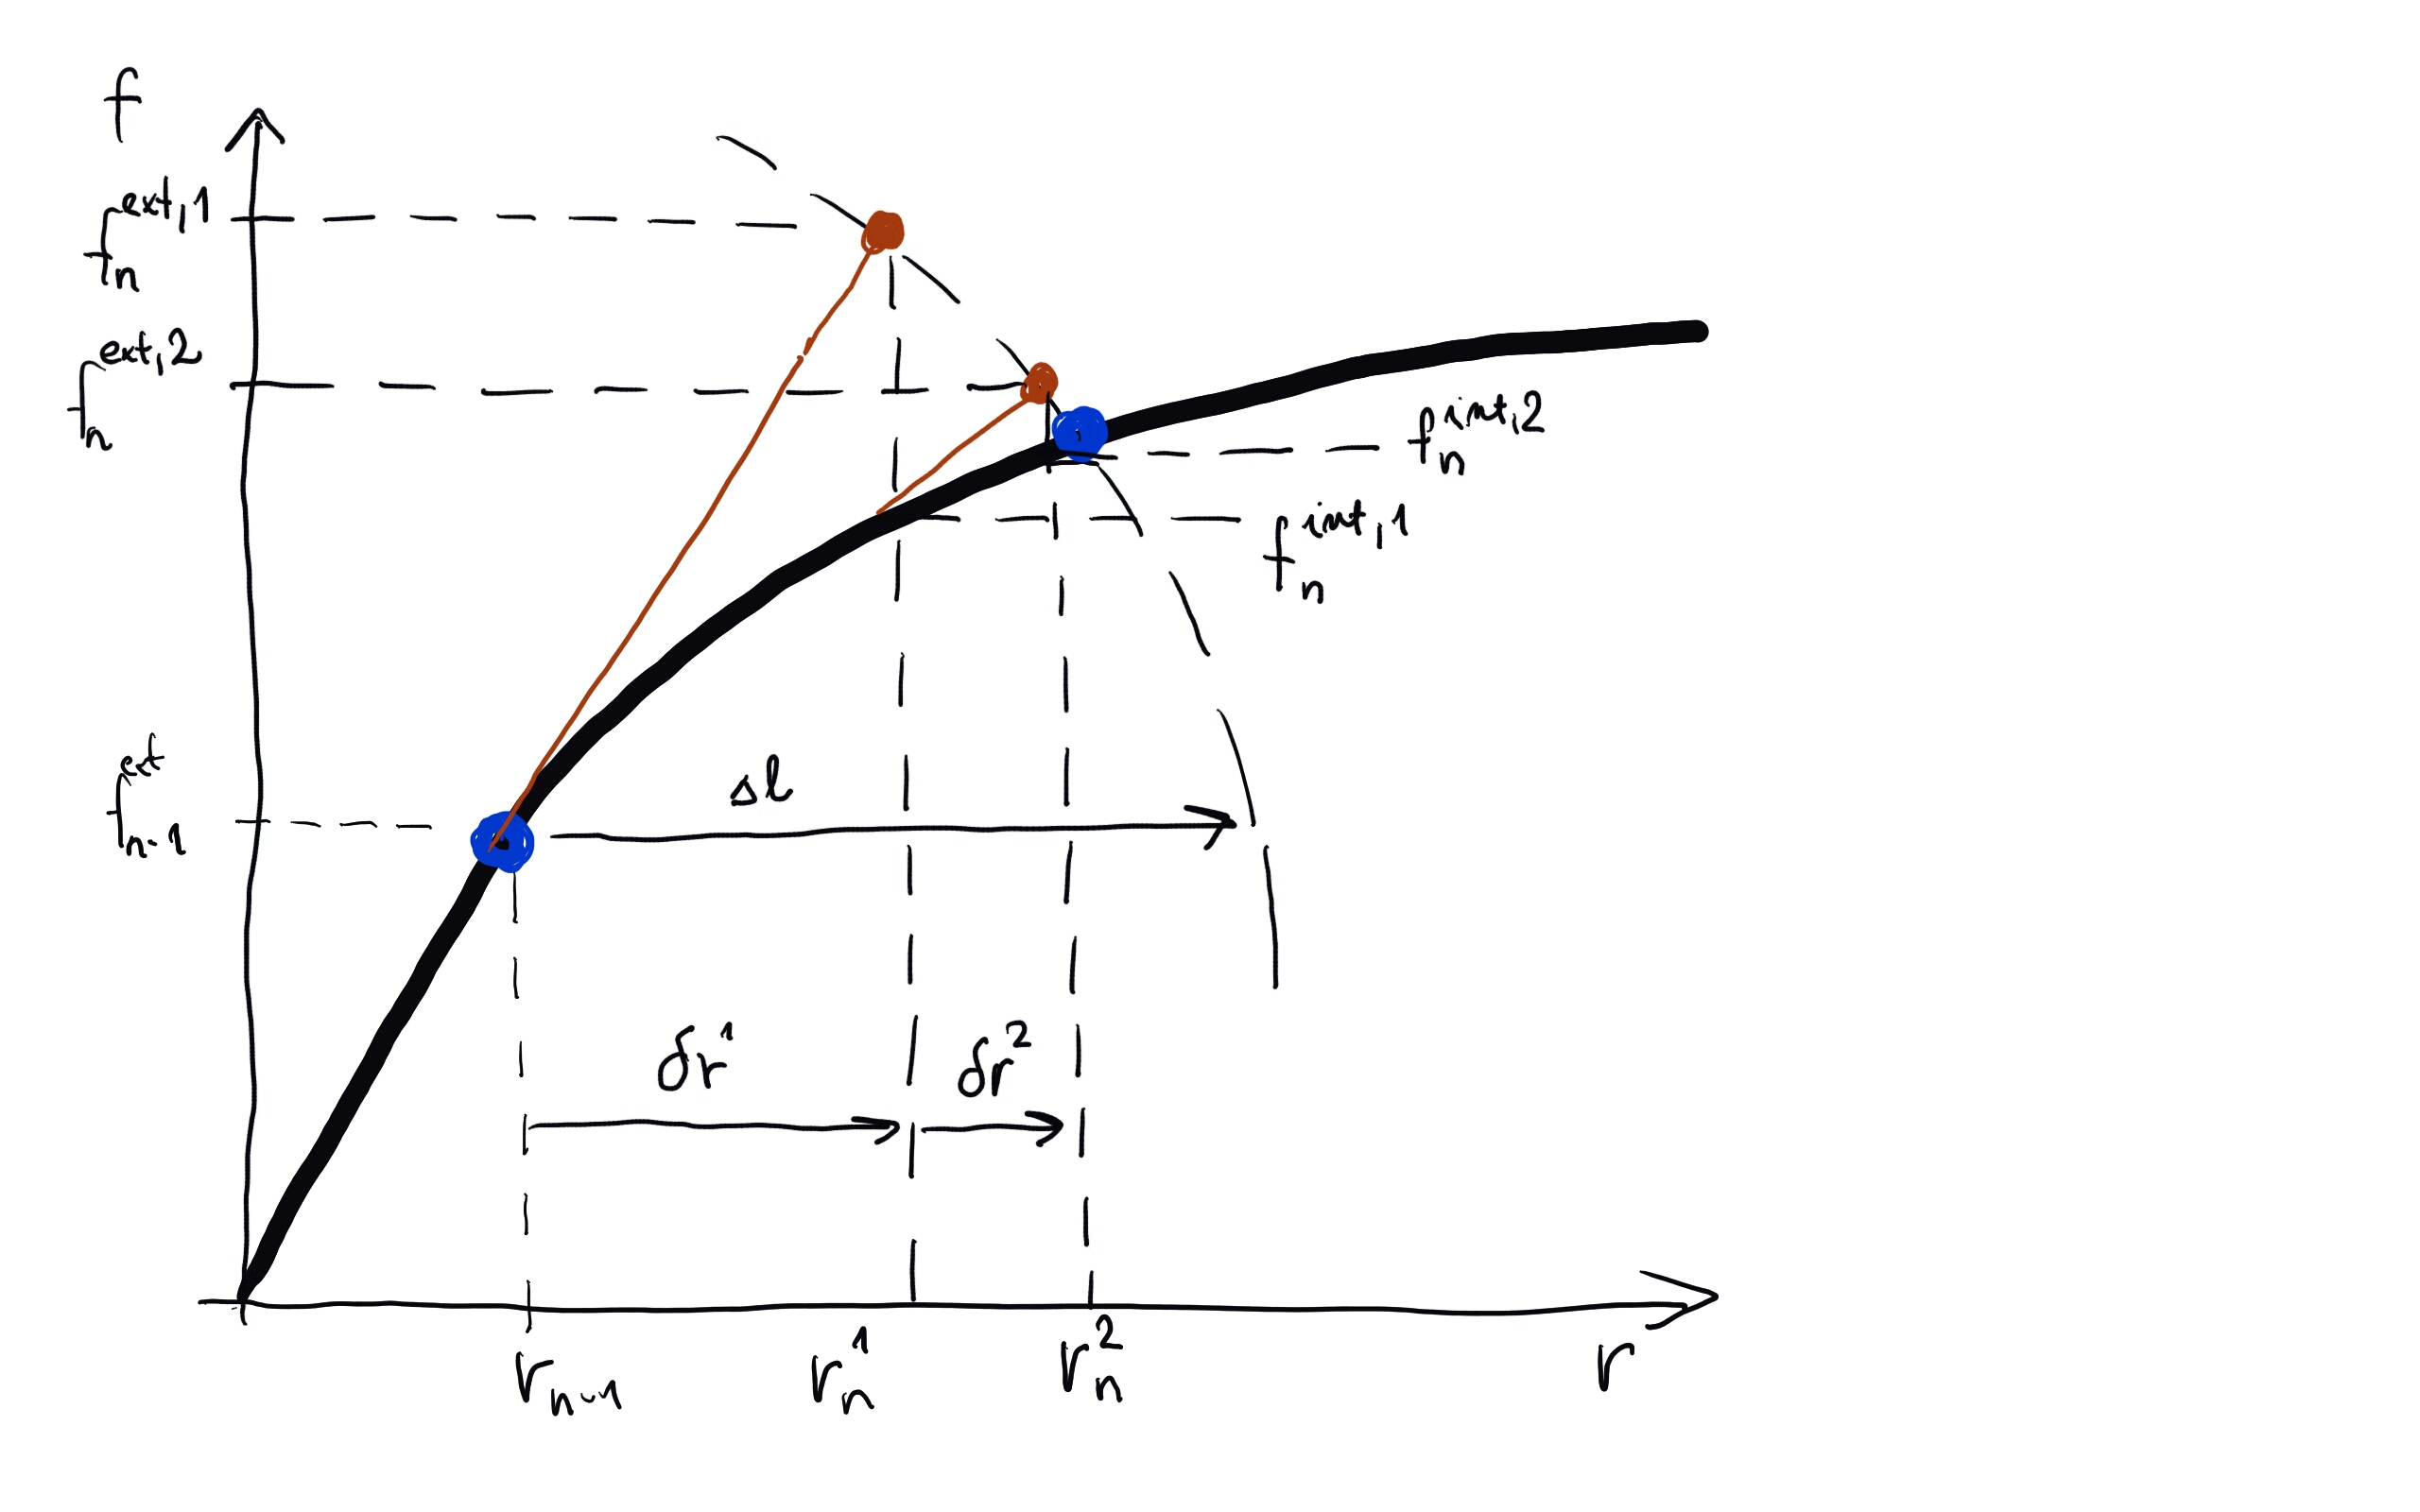
\includegraphics[width=0.8\textwidth]{figs/arclength.png}
  \end{center}
  \label{fig:arclength}
  \caption{Illustration of Acr-length method}
\end{figure}


At the end of n-th loading step and i-th iteration the displacement vector can be written as
$\mbf{r}^i_n = \mbf{r}^{i-1}_n+\delta\mbf{r}$ and similarly the load scaling parameter as $\lambda_n^i = \lambda_n^{i-1}+\delta\lambda$. Substituting this into equilibrium equation~\ref{eq:alm1} we get
$$\mbf{f}^{int}(\mbf{r}_n^{i-1}+\delta\mbf{r})=\mbf{f}^{ext}((\lambda_n^{i-1}+\delta\lambda)\mbf{f}_p)$$
By linearization of $\mbf{F}^{int}$ around known state $\mbf{r}_n^{i-1}$ we get
$$\mbf{f}^{int}_n(\mbf{r}_n^{i-1})+\mbf{K}_n^{i-1}\delta\mbf{r} = \mbf{f}^{ext,i-1}+\delta\lambda\mbf{f}_p$$
and finally for unknown $\delta\mbf{r}$
\begin{equation}
  \delta\mbf{r} = \underbrace{(\mbf{K}_n^{i-1})^{-1}(\mbf{f}^{ext,i-1}-\mbf{f}^{int}(\mbf{r}_n^{i-1}))}_{\delta\mbf{r}_r} + \delta\lambda\underbrace{(\mbf{K}_n^{i-1})^{-1}\mbf{f}_p}_{\delta\mbf{r}_\lambda}
\end{equation}
Note that the vectors $\delta\mbf{r}_r$ and $\delta\mbf{r}_\lambda$ can be computed and the only unknown remaining is the incremental change of loading parameter $\delta\lambda$, which could be determined from~\ref{eq:alm2}
\begin{eqnarray}
  \Delta l_n^2&=&(\Delta\mbf{r}_n^{i-1}+\delta\mbf{r}_r+\delta\lambda\delta\mbf{r}_\lambda)^T(\Delta\mbf{r}_n^{i-1}+\delta\mbf{r}_r+\delta\lambda\delta\mbf{r}_\lambda) + c^2(\Delta\lambda_n^{i-1}+\delta\lambda)^2\mbf{f}^T_p\mbf{f}_p
  \label{eq:quadraticlambda}
\end{eqnarray}
This finally yields a quadratic equation for unknown increment of loading parameter $\delta\lambda$. The algorithm is summarized in Table~\ref{tab:alm}.

\begin{table}[h!]
  \begin{center}
  \begin{tabular}{|l|l|}
    \hline
    Given \\
    \;\;$\mbf{f}^{ext}_{n-1}, \mbf{f}_p$\\
    \;\;$\mbf{r}^{0}_{n} = \mbf{r}_{n-1}$\\
    Evaluate\\
    $\;\;\delta\mbf{r}_\lambda = (\mbf{K}_n)^{-1}\mbf{f}_p$\\
    $\;\;\Delta\lambda^0=\pm{\Delta l}/{\sqrt{\delta\mbf{r}_\lambda^T\delta\mbf{r}_\lambda+c^2\mbf{f}_p^T\mbf{f}_p}}$\\
    $\;\;\Delta\mbf{r}_n^0 = (\mbf{K}_n)^{-1}(\Delta\lambda\mbf{f}_p) = (\mbf{K}_n)^{-1}((\lambda_n+\Delta\lambda^0)\mbf{f}_p - \mbf{f}^{int,0}_n)$\\
    Repeat for $i=1,2,\cdots$\\ 
    $\;\;\delta\mbf{r}_\lambda = (\mbf{K}_n^{i-1})^{-1}\mbf{f}_p$\\
    $\;\;\delta\mbf{r}_r = (\mbf{K}_n^{i-1})^{-1}(\lambda_n^{i-1}\mbf{f}_p-\mbf{f}^{int}(\mbf{r}_n^{i-1}))$\\
    $\;\;$Solve quadratic equation~\ref{eq:quadraticlambda} for $\delta\lambda$\\
    $\;\;\delta\mbf{r}^i = \delta\mbf{r}_r+\delta\lambda\delta\mbf{r}_\lambda$\\
    $\;\;\Delta\mbf{r}_n^i = \Delta\mbf{r}^{i-1}+\delta\mbf{r}^i,\ \mbf{r}_n^i = \mbf{r}_n^{i-1}+\delta\mbf{r}^i$\\
    $\;\;\lambda^i = \lambda^{i-1}+\delta\lambda,\ \Delta\Lambda_n^i = \Delta\Lambda_n^{i-1}+\delta\lambda$\\
    Until convergence reached\\
    \hline
  \end{tabular}
  \end{center}
  \caption{Newton-Raphson method}
  \label{tab:newtonraphson}
\end{table}












\section{Non-stationary linear transport model}
\label{NonLinTrans}
The weak form of diffusion-type differential equation leads to
\begin{eqnarray}
\mbf{K} \mbf{r} + \mbf{C}\frac{{\rm d}\mbf{r}}{{\rm d} t} = \mbf{F}\label{NonLinTrans:1},
\end{eqnarray}
where the matrix $\mbf{K}$ is a general non-symmetric conductivity matrix, $\mbf{C}$ is a general capacity matrix and the vector $\mbf{F}$ contains contributions from external and internal sources. The vector of unknowns, $\mbf{r}$, can hold nodal values of temperature, humidity, or concentration fields, for example.

Time discretization is based on a generalized trapezoidal rule. Let us assume that the solution is known at time $t$ and the time increment is $\Delta t$. The parameter $\alpha\in\langle 0, 1\rangle$ defines a type of integration scheme; $\alpha=0$ results in an explicit (forward) method, $\alpha=0.5$ refers to the Crank-Nicolson method, and $\alpha=1$ means an implicit (backward) method. The appromation of solution vector and its time derivative yield
\begin{eqnarray}
\tau &=& t+\alpha\Delta t = (t+\Delta t) - (1-\alpha)\Delta t,\label{NonLinTrans:2}\\
\mbf{r}_{\tau} &=& (1-\alpha)\mbf{r}_t+\alpha\mbf{r}_{t+\Delta t},\label{NonLinTrans:3}\\
\frac{{\rm d}\mbf{r}}{{\rm d} t} &=& \frac{1}{\Delta t}\left(\mbf{r}_{t+\Delta t}-\mbf{r}_t\right).\label{NonLinTrans:4}\\
\mbf{F}_{\tau} &=& (1-\alpha)\mbf{F}_t+\alpha\mbf{F}_{t+\Delta t},\label{NonLinTrans:5}
\end{eqnarray}

Let us assume that \refeq{NonLinTrans:1} should be satisfied at time $\tau$. Inserting \refeqsr{NonLinTrans:3}{NonLinTrans:5}
into \refeq{NonLinTrans:1} leads to
\begin{eqnarray}
\left[\alpha \mbf{K} + \frac{1}{\Delta t} \mbf{C} \right] \mbf{r}_{t+\Delta t} = 
\left[(\alpha-1) \mbf{K} + \frac{1}{\Delta t} \mbf{C} \right] \mbf{r}_{t} +
(1-\alpha) \mbf{F}_{t} + \alpha \mbf{F}_{t+\Delta t}\label{NonLinTrans:6}
\end{eqnarray}
where the conductivity matrix $\mbf{K}$ contains also a contribution from convection, since it depends on
$\mbf{r}_{t+\Delta t}$
\begin{eqnarray}
\mbf{K} = \int_{\Omega}\mbf{B}^T \lambda \mbf{B} \ud\Omega + \underbrace{\int_{{\Gamma}_{\overline{c}}} \mbf{N}^T h \mbf{N} \ud \Gamma}_{\textrm{Convection}}\label{NonLinTrans:7}
\end{eqnarray}
The vectors $\mbf{F}_t$ or $\mbf{F}_{t+\Delta t}$ contain all known contributions
\begin{eqnarray}
\mbf{F}_t = - \underbrace{\int_{\Gamma_{\overline{q}}} \mbf{N}^T \overline{q}_t \ud \Gamma}_{\textrm{Given flow}} +
\underbrace{\int_{\Gamma_{\overline{c}}} \mbf{N}^T h T_{\infty,t} \ud \Gamma}_{\textrm{Convection}} +
\underbrace{\int_{\Omega}\mbf{N}^T\overline{Q}_t\ud\Omega}_{\textrm{Source}}\label{NonLinTrans:8}
\end{eqnarray}

\section{Non-stationary nonlinear transport model}
\label{NonNonTrans}
In a nonlinear model, \refeq{NonLinTrans:1} is modified to
\begin{eqnarray}
\mbf{K}(\mbf{r}) \mbf{r} + \mbf{C}(\mbf{r})\frac{{\rm d}\mbf{r}}{{\rm d} t} = \mbf{F}(\mbf{r})\label{NonNonTrans:1},
\end{eqnarray}

Time discretization is the same as in \refeqsr{NonLinTrans:2}{NonLinTrans:4} but the assumption in \refeq{NonLinTrans:8} is not true anymore. Let us assume that \refeq{NonNonTrans:1} should be satisfied at time $\tau\in\langle t,t+\Delta t \rangle$. By substituting of \refeqsr{NonLinTrans:3}{NonLinTrans:4} into \refeq{NonNonTrans:1} leads to the following equation
\begin{equation}
\left[(1-\alpha)\mbf{r}_t + \alpha\mbf{r}_{t+\Delta t} \right] \mbf{K}_{\tau}(\mbf{r}_\tau) +
\left[\del{\mbf{r}_{t+\Delta t}-\mbf{r}_t}{\Delta t}\right] \mbf{C}_{\tau}(\mbf{r}_\tau) = 
\mbf{F}_{\tau}(\mbf{r}_\tau).\label{NonNonTrans:5}
\end{equation}

\refeq{NonNonTrans:5} is non-linear and the Newton method is used to obtain the solution. First, the \refeq{NonNonTrans:5} is 
transformed into a residual form with the residuum vector $\mbf{R}_{\tau}$, which should converge to the zero vector
\begin{equation}
\mbf{R}_{\tau} = 
\left[(1-\alpha)\mbf{r}_t + \alpha\mbf{r}_{t+\Delta t} \right] \mbf{K}_{\tau}(\mbf{r}_\tau) +
\left[\del{\mbf{r}_{t+\Delta t}-\mbf{r}_t}{\Delta t}\right] \mbf{C}_{\tau}(\mbf{r}_\tau) -
\mbf{F}_{\tau}(\mbf{r}_\tau) \to \mbf{0}.\label{NonNonTrans:6}
\end{equation}

A new residual vector at the next iteration, $\mbf{R}_\tau^{i+1}$, can determined from the previous residual vector, $\mbf{R}_{\tau}^i$, and its derivative simply by linearization. Since the aim is getting an increment of solution vector, $\Delta\mbf{r}_{\tau}^i$, the new residual vector $\mbf{R}_{\tau}^{i+1}$ is set to zero
\begin{eqnarray}
\mbf{R}_\tau^{i+1} &\approx& \mbf{R}_{\tau}^i+\frac{\partial{\mbf{R}_{\tau}^i}}{\partial\mbf{r}_t} \Delta\mbf{r}_{\tau}^i = \mbf{0},\label{NonNonTrans:7}\\
\Delta \mbf{r}_{\tau}^i &=& - \left[\frac{\partial{\mbf{R}_{\tau}^i}}{\partial\mbf{r}_t}\right]^{-1} \mbf{R}_{\tau}^i\label{NonNonTrans:8}.
\end{eqnarray}
Deriving \refeq{NonNonTrans:6} and inserting to \refeq{NonNonTrans:8} leads to
\begin{eqnarray}
\mbf{\tilde K}_\tau^i &=& \frac{\partial{\mbf{R}_{\tau}^i}}{\partial\mbf{r}_t} = -\alpha \mbf{K}_{\tau}^i(\mbf{r}) - \del{1}{\Delta
t}\mbf{C}_{\tau}^i(\mbf{r})\label{NonNonTrans:9},\\
\Delta \mbf{r}_{\tau}^i &=& - \left[\mbf{\tilde K}_\tau^i\right]^{-1} \mbf{R}_{\tau}^i,\label{NonNonTrans:10}
\end{eqnarray}
which gives the resulting increment of the solution vector $\Delta \mbf{r}_{\tau}^i$
\begin{equation}
\begin{split}
\Delta \mbf{r}_{\tau}^i = - \left[\mbf{\tilde K}_\tau^i\right]^{-1} \Big\{ &\left[(1-\alpha)\mbf{r}_t + \alpha\mbf{r}_{t+\Delta t} \right] \mbf{K}_{\tau}^i(\mbf{r}_\tau) +\\
&\left[\del{\mbf{r}_{t+\Delta t}-\mbf{r}_t}{\Delta t}\right] \mbf{C}_{\tau}^i(\mbf{r}_\tau) - \mbf{F}_{\tau}(\mbf{r}_\tau) \Big\},\label{NonNonTrans:11}
\end{split}
\end{equation}
and the new total solution vector at time $t + \Delta t$ is obtained in each iteration
\begin{eqnarray}
\mbf{r}_{t+\Delta t}^{i+1}=\mbf{r}_{t+\Delta t}^{i} + \Delta\mbf{r}_{\tau}^i.\label{NonNonTrans:12}
\end{eqnarray}

There are two options how to initialize the solution vector at time $t + \Delta t$. While the first case applies linearization with a known derivative, the second case simply starts from the previous solution vector. The second method in \refeq{NonNonTrans:14} is implemented in OOFEM.
\begin{eqnarray}
\mbf{r}_{t+\Delta t}^{0} = \mbf{r}_t + \Delta t\frac{\partial{\mbf{r}_t}}{\partial t},\label{NonNonTrans:13}\\
\mbf{r}_{t+\Delta t}^{0} = \mbf{r}_t.\label{NonNonTrans:14}
\end{eqnarray}

Note that the matrices $\mbf{K}(\mbf{r}_\tau), \mbf{C}(\mbf{r}_\tau)$ and the vector $\mbf{F}(\mbf{r}_\tau)$ depend on the solution vector $\mbf{r}_\tau$. For this reason, the matrices are updated in each iteration step (Newton method) or only after several steps (modified Newton method). The residuum $\mbf{R}_\tau^{i}$ and the vector $\mbf{F}_\tau(\mbf{r}_\tau)$ are updated in each iteration, using the most recent capacity and conductivity matrices.

\subsection{Heat flux from radiation}

Heat flow from a body surrounded by a medium at a temperature $T_\infty$ is governed by the Stefan-Boltzmann Law
\begin{eqnarray}
q(T, T_\infty) = \varepsilon \sigma (T^4 - T_\infty^4)\label{eq:StefanBoltzmann}
\end{eqnarray}
where $\varepsilon\in\langle 0, 1 \rangle$ represents emissivity between the surface and the boundary at temperature $T_\infty$. $\sigma=5.67\cdot 10^{-8}$ W/m$^{-2}$K$^{-4}$ stands for a Stefan-Boltzmann constant. Transport elements in OOFEM implement \refeq{eq:StefanBoltzmann} and require non-linear solver.

Alternatively (not implemented), a linearization using Taylor expansion around $T_\infty$ and neglecting higher-order terms results to
\begin{eqnarray}
q(T, T_\infty) &\approx& q(T=T_\infty) + \frac{\partial q(T,T_\infty)}{\partial T_\infty} (T_\infty-T) = 4\varepsilon \sigma T_\infty^3 (T-T_\infty)
\end{eqnarray}
leading to so-called radiation heat transfer coefficient $\alpha_{rad}=4\varepsilon \sigma T_\infty^3$. The latter resembles similar coefficient as in convective heat transfer. Other methods for \refeq{eq:StefanBoltzmann} could be based on Oseen or Newton-Kantorovich linearization. Also, radiative heat transfer coefficient $\alpha_{rad}$ can be expressed as \cite[pp.28]{Baehr:06}
\begin{eqnarray}
q(T, T_\infty) = \varepsilon \sigma \frac{T^4 - T_\infty^4}{T-T_\infty}(T-T_\infty) = \underbrace{\varepsilon \sigma (T^2+T_\infty^2)(T+T_\infty)}_{\alpha_{rad}}(T-T_\infty)
\end{eqnarray}



\section{Transient incompressible flow - Lagrangian Particle Method}
\subsection{Lagrangian governing equations of incompressible fluid}
The Particle finite element method (PFEM) is based on the Lagrangian form of the Navier-Stokes equation for incompressible Newtonian fluids. Assuming the density does not change in time for an incompressible fluid, the continuity equation reduces to zero requirements for the divergence of the velocity. The Navier-Stokes equations take the form
\begin{eqnarray}
\rho\pard{\mbf{u}}{t} &=& \rho\mbf{b} + \nabla\cdot\mbf{\sigma} \label{eq:navier-stokes2}\;,\\
\nabla\cdot\mbf{u} &=& 0\;. \label{eq:navier-stokes2b}
\end{eqnarray}
For the deviatoric stress in Newtonian fluids a linear dependency of stress tensor and strain rate tensor is adopted and for the Newtonian fluids. Considering the incompressibility of the fluid, the Cauchy stress reads
\begin{equation}\label{eq:stokes}
\mbf{\sigma}=-p\mbf{I} + 2\mu \nabla^s\mbf{u}\;.
\end{equation}
This equation is known as \emph{Stokes' law} and its Cartesian form writes
\begin{equation}
\sigma_{ij}=-p\delta_{ij}+\mu\left(\pard{u_i}{x_j}+\pard{u_j}{x_i}\right)\;.
\end{equation}
\par
Substituting the expression of Cauchy stress from Stokes' law~(\ref{eq:stokes}) into the momentum equation~(\ref{eq:navier-stokes2}) and rewriting gives
\begin{equation}
\rho\pard{\mbf{u}}{t} = \rho\mbf{b} + \mu\nabla^2\mbf{u} - \nabla p\;.\label{eq:momentum}
\end{equation}
\par
The governing equations of the mass~(\ref{eq:navier-stokes2b}) and momentum conservation~(\ref{eq:momentum}) form can be written in the Cartesian form for the individual component $i$ using Einstein summation convention
\begin{eqnarray}
\rho \pard{u_i}{t} &=& - \frac{\partial}{\partial x_i}p+\mu\frac{\partial}{\partial x_j}\left(\frac{\partial u_i}{\partial x_j}\right)+\rho b_i \;, \label{eq:mb}\\
\pard{u_i}{x_i} &=& 0\;.
\end{eqnarray}
The equations are accompanied by a set of standard boundary conditions imposed on the complementary parts of the domain boundary
\begin{eqnarray}
  \tau_{ij}\nu_j - p\nu_i &=& \bar \sigma_{ni} \qquad \mbox{on } \Gamma_{\sigma}\;, \\
  u_i\nu_i &=& \bar u_n \qquad\; \mbox{on } \Gamma_n\;, \\
  u_i\zeta_i &=& \bar u_t \qquad\;\, \mbox{on } \Gamma_t\;,
\end{eqnarray}
where $\nu$ or $n$ denotes the normal direction to the boundary and $\zeta$ or $t$ the tangential one. The bar sign over a quantity $\bar x$ stands for its prescribed value.

\subsection{Time discretization}
For the time discretization of the momentum equation, a general trapezoid rule can be adopted. Using this rule, the time derivative of a generic function $\phi$ can be approximated by following equation
\begin{equation}
[\phi(x,t)]^{n+\theta} = \theta\phi(x,t^{n+1})+(1-\theta)\phi(x,t^n)=\theta\phi^{n+1}+(1-\theta)\phi^n\;.
\end{equation}
Rewriting the time derivative on the left hand side of the momentum balance~(\ref{eq:mb}) as a finite difference in time and applying the trapezoidal rule on the right hand side, we obtain
\begin{equation}\label{eq:momentum-general}
  \rho\pard{u_i}{t} \approx \rho\frac{u^{n+1}_i-u^n_i}{\Delta t}= \left[ - \frac{\partial}{\partial x_i}p+\mu\frac{\partial}{\partial x_j}\left(\frac{\partial u_i}{\partial x_j}\right)+\rho b_i\right]^{n+\theta}\;.
\end{equation}
The parameter $\theta$ can take values from the interval $[0,1]$.  The approximation is considered as a weighted average of the derivative values in the time step $n$ and $n+1$. Using a specific value of the $\theta$ parameter, well-known methods can be recovered: The explicit Euler method $\theta=0$, the backward Euler for $\theta=1$ or the Crank-Nicolson method $\theta=1/2$. The current implemantation of PFEM allows the use of explicit and backward (implicit) method.

\subsection{Fractional step scheme}
Beside the three velocity components, the discretized momentum balance equations~(\ref{eq:momentum-general}) for a three dimensional case includes pressure as a coupling variable. A possible approach to decouple them is the application of so-called \emph{fractional step method}. The main idea of this method consists in introducing an intermediate velocity as supplementary variable and splitting the momentum equation. The modification introduced by R.Codina~\cite{Codina01} splits the the discretized time step is split into two sub-steps. The implicit part of the pressure is avoided and assigned to the second step.
\begin{equation}
  \pard{u_i}{t} \approx \frac{u^{n+1}_i-u^n_i}{\Delta t}=\frac{u^{n+1}_i-u^*_i+u^*_i-u^n_i}{\Delta t}= \left[ - \frac{1}{\rho}\frac{\partial}{\partial x_i}p+\frac{\mu}{\rho}\frac{\partial}{\partial x_j}\left(\frac{\partial u_i}{\partial x_j}\right)+b_i\right]^{n+\theta}\;.
\end{equation}
where the intermediate velocity $u^*_i$ is introduced. Splitting the equation in the following manner gives the expression for the unknown velocities
\begin{eqnarray}\label{rce:uistar}
    u^*_i &=& u^n_i+b_i\Delta t - \frac{\Delta t}{\rho}\pard{}{x_i}\gamma p^n+\frac{\Delta t\mu}{\rho}\pard{}{x_j}\left(\pard{u^{n+\theta}_i}{x_j}\right)\;,\\
    u^{n+1}_i &=& u^*_i- \frac{\Delta t}{\rho}\pard{}{x_i}(p^{n+1}-\gamma p^n)\;. \label{eq:uin1}
\end{eqnarray}

The pressure split is here introduced by the new parameter $\gamma$ defining the amount of splitting and can take values from 0 to 1. The body loads are considered to be constant over time step.
\par
In a similar way, the fractional step method is applied on the mass conservation equation. Here, the time derivative of density would be approximated. As we examine an incompressible flow, whose density does not change in time, merely the intermediate velocity term is incorporated in the divergence of the velocity.
\begin{equation}
  \pard{(u^{n+1}_i-u^*_i+u^*_i)}{x_i} = 0 \;,
\end{equation}
which can be decomposed into two sub-equations

\begin{eqnarray}\label{rce:mass}
	\pard{u^*_i}{x_i} &=& 0 \\
      \pard{(u^{n+1}_i-u^*_i)}{x_i} &=& 0\;.
\end{eqnarray}

By substituting for the velocity difference into the equation~(\ref{eq:uin1}) we obtain
\begin{equation}
\pard{}{x_i}(u^{n+1}_i - u^*_i) = \pard{}{x_i}\left(-\frac{\Delta t}{\rho}\pard{}{x_i}(p^{n+1}-\gamma p^n)\right)\;.
\end{equation}
Now we can sum the separated mass equations together. This operation gives the coupled mass-momentum equation
\begin{equation}
  \pard{u^*_i}{x_i} - \frac{\Delta t}{\rho}\frac{\partial^2}{\partial x^2_i}(p^{n+1}-\gamma p^n) = 0\;.
\end{equation}
The final set of equations reads
\begin{eqnarray}
u^*_i  &=& u^n_i+b_i\Delta t - \frac{\Delta t}{\rho}\pard{}{x_i}\gamma p^n+\frac{\Delta t\mu}{\rho}\pard{}{x_j}\left(\pard{u^{n+\theta}_i}{x_j}\right)\;,\\
\frac{\partial^2}{\partial x^2_i}(p^{n+1}) &=& \frac{\rho}{\Delta t}\pard{u^*_i}{x_i}+\frac{\partial^2}{\partial x^2_i}(\gamma p^n)\;, \\
u^{n+1}_i &=& u^*_i- \frac{\Delta t}{\rho}\pard{}{x_i}(p^{n+1}-\gamma p^n)\;.
\end{eqnarray}
\par
The above PFEM formulation is based on the paper by Idelsohn, O\~nate and Del Pin~\cite{Idelsohn04}. The authors described an approach using arbitrary time discretization scheme and pressure split factor. Their choice of implicit scheme $\theta = 1$ was motivated by better convergence properties, whereas the decision for $\gamma = 0$ leading to greater pressure split was driven by better pressure stabilization.
\subsection{Spatial discretization}
The unknown functions of velocity and pressure are approximated using equal order interpolation for all variables in the final configuration
\begin{eqnarray}
u_i&=&\mbf{N}^T(X,t)\mbf{U}_i\\
p&=&\mbf{N}^T(X,t)\mbf{P} \;.
\end{eqnarray}
By applying the Galerkin weighted residual method on the splitted governing equations, following system of linear algebraic equations is obtained 
\begin{eqnarray}
\mbf{M}\mbf{U}^* &=& \mbf{M}\mbf{U}^n + \Delta t\mbf{F} - \frac{\Delta t\mu}{\rho}\mbf{K}\mbf{U}^{n+\theta}\;,\label{eq:systemA} \\
\mbf{L}\mbf{P}^{n+1} &=&\frac{\rho}{\Delta t}\left(\mbf{G}^T\mbf{U}^*-\hat{\mbf{U}}\right) \;, \label{eq:systemB} \\
\mbf{M}\mbf{U}^{n+1} &=& \mbf{M}\mbf{U}^* - \frac{\rho}{\Delta t}\mbf{G}\mbf{P}^{n+1} \;.\label{eq:systemC}
\end{eqnarray}
\par
The matrix $\mbf{M}$ denotes the mass matrix in a lumped form, whereas the vector $\mbf{F}$ stands for the load vector. The matrix $\mbf{G}$ represents the gradient operator, which is the transposition of the divergence operator denoted simply as $\mbf{G}^T$. Matrices $\mbf{K}$ and $\mbf{L}$ are build in a similar way however noted differently. Both mean the Laplacian operator. Due to its common use in computational mechanics, the classical notation of the stiffness matrix $\mbf{K}$ is used. Prescribed velocity components are enclosed in vector $\hat{\mbf{U}}$.
\par
In each computational time step, an iteration is performed until the equilibrium is reached. Depending on the value of $\theta$ used, the equation system for the components of the auxiliary velocity $U^*_i$~(\ref{eq:systemA}) can be solved either explicitly $\theta = 0$ or implicitly $\theta \neq 0$. Then, the calculated values of the auxiliary velocity are used as input for the pressure computation~(\ref{eq:systemB}). The last system of equations~(\ref{eq:systemC}) determines the velocity values at the end of the time step, taking auxiliary velocities and pressure or pressure increments into account.
\par
Let us summarize the iterative step. The position of the particles at the end of the previous time step is known, as well as the the value of the velocity $u^n$ and pressure $p^n$. The set of governing equations is build up for the unknowns at the end of the solution step $\theta^{n+1}$, however based on the geometry of the previous step. The changes in the position are neglected. Once the convergence is reached, the final position is computed from the old one modified by the displacement due to obtained velocity. After that, solution can proceed to the next time step.
